%%%% CAPÍTULO 1 - INTRODUÇÃO
%%
%% Deve apresentar uma visão global da pesquisa, incluindo: breve histórico, importância e justificativa da escolha do tema,
%% delimitações do assunto, formulação de hipóteses e objetivos da pesquisa e estrutura do trabalho.

%% Título e rótulo de capítulo (rótulos não devem conter caracteres especiais, acentuados ou cedilha)
\chapter{Introduction}\label{cap:introducao}

\section{Motivation}

With the advancement of high speed mobile networks and smartphone penetration,
customer demands are on an ever increasing trajectory for more personalized and
digital experiences. Companies worldwide are fighting for customer attention in 
the digital era by developing products and services that bring state-of-the-art 
technologies to the masses in the so called smart devices and systems \cite{Shafique2020}.

As an example of such advancements, smart speakers such as the Amazon Echo
\cite{GaoPanWangChen2018}, shown on Figure \ref{fig:echodot4}, include the latest and greatest in terms of Natural
Language Processing and Deep Learning \cite{Young2018}, allowing customers to
interact with the product in an conversational manner that was considered to be
science fiction material until a couple of years ago.

\begin{figure}[!htb]
	\centering
	\caption[Amazon Echo 4th Generation smart speaker promotional material]{Amazon Echo 4th Gen Smart Speaker promotional material}
	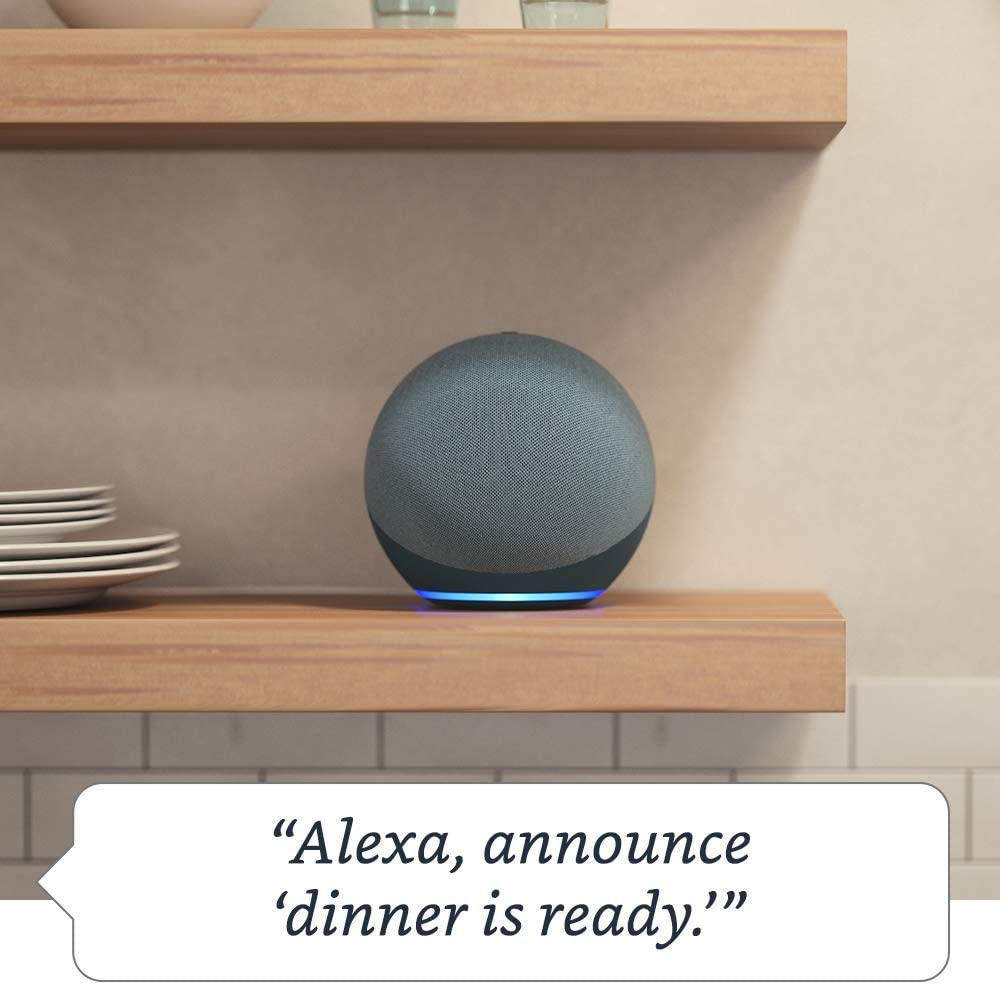
\includegraphics[width=0.4\textwidth]{./images/echodot4.jpg} % <- formatos PNG, JPG e PDF
    \fonte{Amazon (2022)}
	\label{fig:echodot4}
\end{figure}

\begin{quote}
    \textit{This device is a gem! When I’m busy in the kitchen, for example, and can’t get
    to a computer to find info or music to play, Alexa would be there to listen
    and do what I ask.} \\
    Customer review from \cite{GaoPanWangChen2018}
\end{quote}

Alongside the devices themselves, entirely new markets have emerged such as the
third-party software extensions called \textit{Alexa Skills} \cite{Alexa2022}.

These skills function much like mobile phone apps, extending and enhancing the
functionality of the device and can be sold to end users.

Developers can then easily leverage the highly advanced machine learning models
through Application Programming Interfaces (\sigla{API}{Application Programming
Interface}) and focus exclusively on their business logic, as shown on Figure
\ref{fig:alexaskill}.

This can be valuable as Machine Learning models are considered to be
expensive to develop and maintain, with some sources mentioning a minimum expenditure 
of US\$ 60.000 over a five year period considering both tasks \cite{Phdata2021}.

\begin{figure}[htb!]
	\centering
	\caption[Diagram showing the steps of an interaction with an Alexa Skill]{Diagram showing the steps of an interaction with an Alexa Skill}
	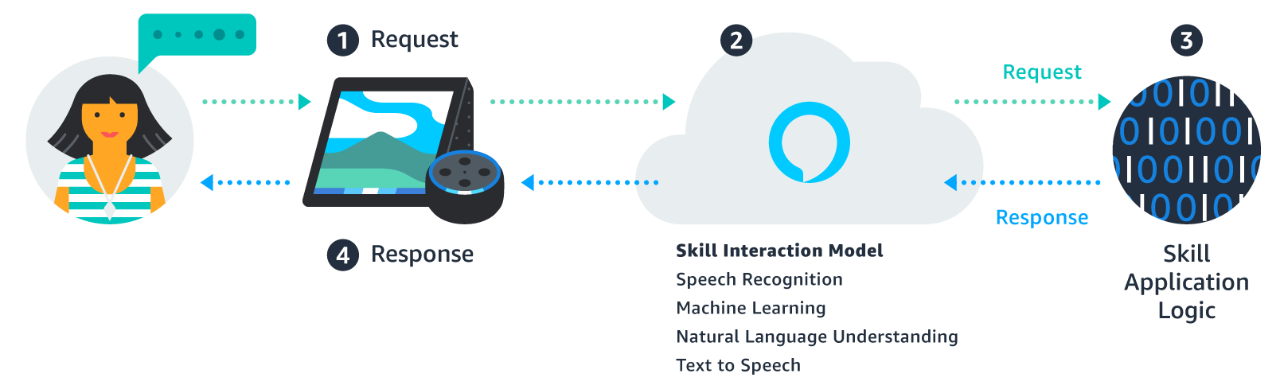
\includegraphics[width=0.9\textwidth]{./images/skills.png} % <- formatos PNG, JPG e PDF
    \fonte{\cite{Alexa2022}}
	\label{fig:alexaskill}
\end{figure}

More impressively, such technological advancements have been able to reach a
considerable amount of households in a short period of time in developed
countries like the United States, as shown on Figure \ref{fig:smartspeaker}.

\begin{figure}[H]
	\centering
	\caption[US Smart Speaker Penetration from 2017 to 2022]{US Smart Speaker Penetration from 2017 to 2022}
	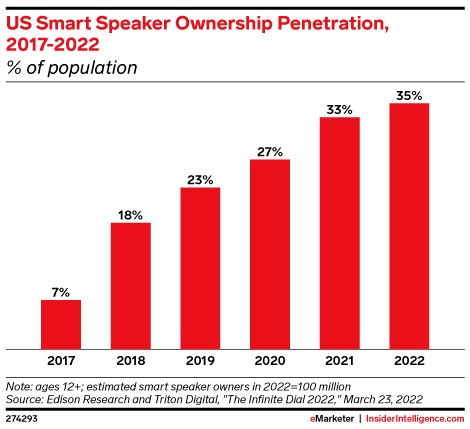
\includegraphics[width=0.6\textwidth]{./images/smartspeaker.png} % <- formatos PNG, JPG e PDF
    \fonte{\cite{InsiderIntelligence2022}}
	\label{fig:smartspeaker}
\end{figure}

On developing countries such as Brazil, these innovations tend to
have delayed arrivals due to historical economic barriers but the potential
customer base has attracted big tech companies like Amazon, which are able
to shorten the arrival delay with their economic power.

In Figure \ref{fig:alexabr}, we can see an example of a smart speaker advertisement 
from Amazon for the Brazilian customer base.

\begin{figure}[h!]
	\centering
	\caption[Localized promotional material for the Echo Show 10 targeting Brazilian customers]{Localized promotional material for the Echo Show 10 targeting Brazilian customers}
	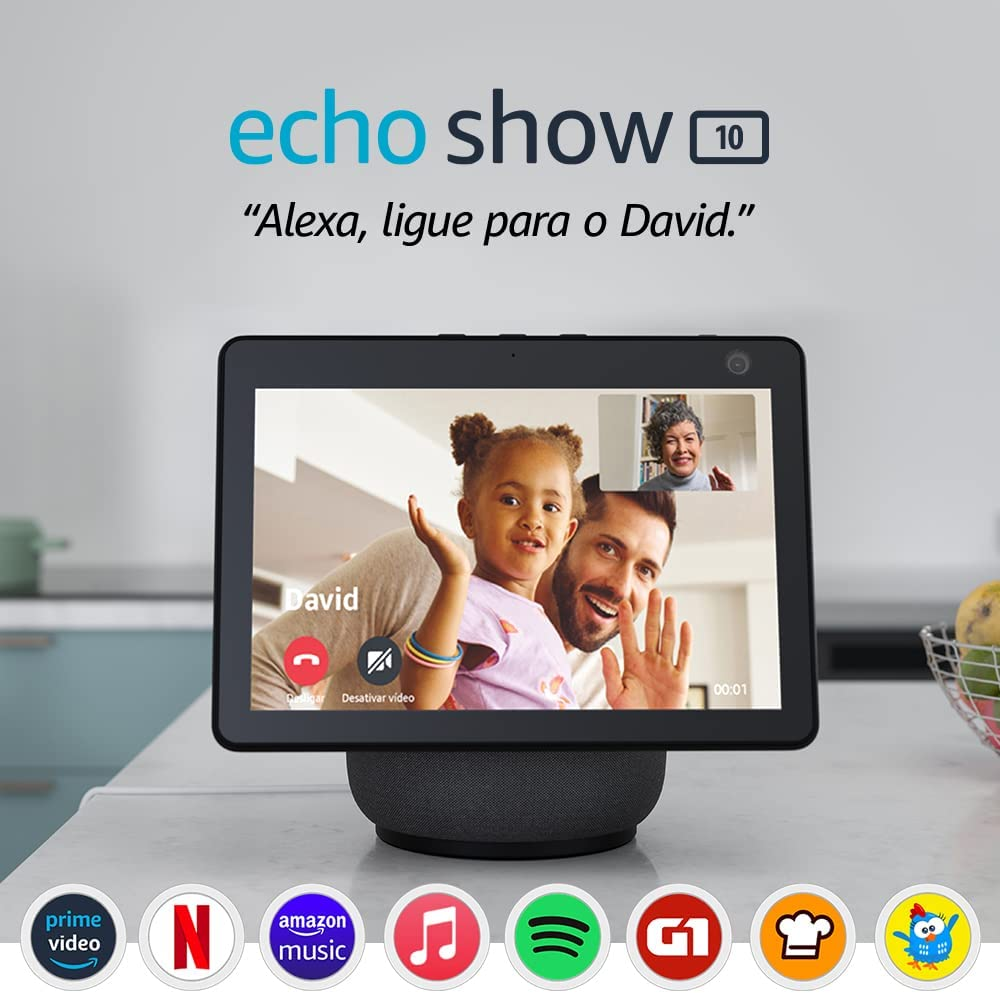
\includegraphics[width=0.4\textwidth]{./images/alexabr.jpg} % <- formatos PNG, JPG e PDF
    \fonte{Amazon (2022)}
    \label{fig:alexabr}
\end{figure}

According to the research company IDC Brasil, the Brazilian home automation
market -- in which smart speakers are included -- would have reached US\$ 291
million on 2021, an impressive figure that might explain the attractiveness of
our market \cite{IDCBrasil}.

But even with all of these innovations impacting customer behaviors day by day, one
important aspect of consumer life still has not had any significant changes in
the last couple of years: \textbf{shopping on
physical stores}.

According to \sigla{ABRAS}{Associação Brasileira de Supermercados} - the
Brazilian Supermarket Association - the Brazilian grocery retail sector has reached an
impressive total revenue of \textbf{R\$ 611 billion} in 2021 - roughly US\$ 117 billion on
October 2022 conversion rates - making up 7,03\% of the national \sigla{GDP}{Gross
Domestic Product}. About \textbf{28 million} customers visit one of the more than
\textbf{92.000} stores countrywide on a daily basis \cite{Abras2022}.

Despite all the technological advancement seen over the last few years and the
economic relevance of such sector, retail grocery shopping still exhibits the
same limitations found a decade ago. In a survey conducted in 2019, Capgemini
has found out five key pain problems related to physical stores in general
\cite{Capgemini2020}:

\begin{enumerate}
        \item Long queues for payment checkout
        \item Out of stock products
        \item Difficulties in locating products in the store
        \item Not being able to find a store associate to help
        \item Lack of product information when I select products
\end{enumerate}

The survey results can be seen in more detail in Figure \ref{fig:capgemini}.

\begin{figure}[H]
	\centering
    \caption[Top five customer pain points in retail stores]{Top five customer pain points in retail stores}
	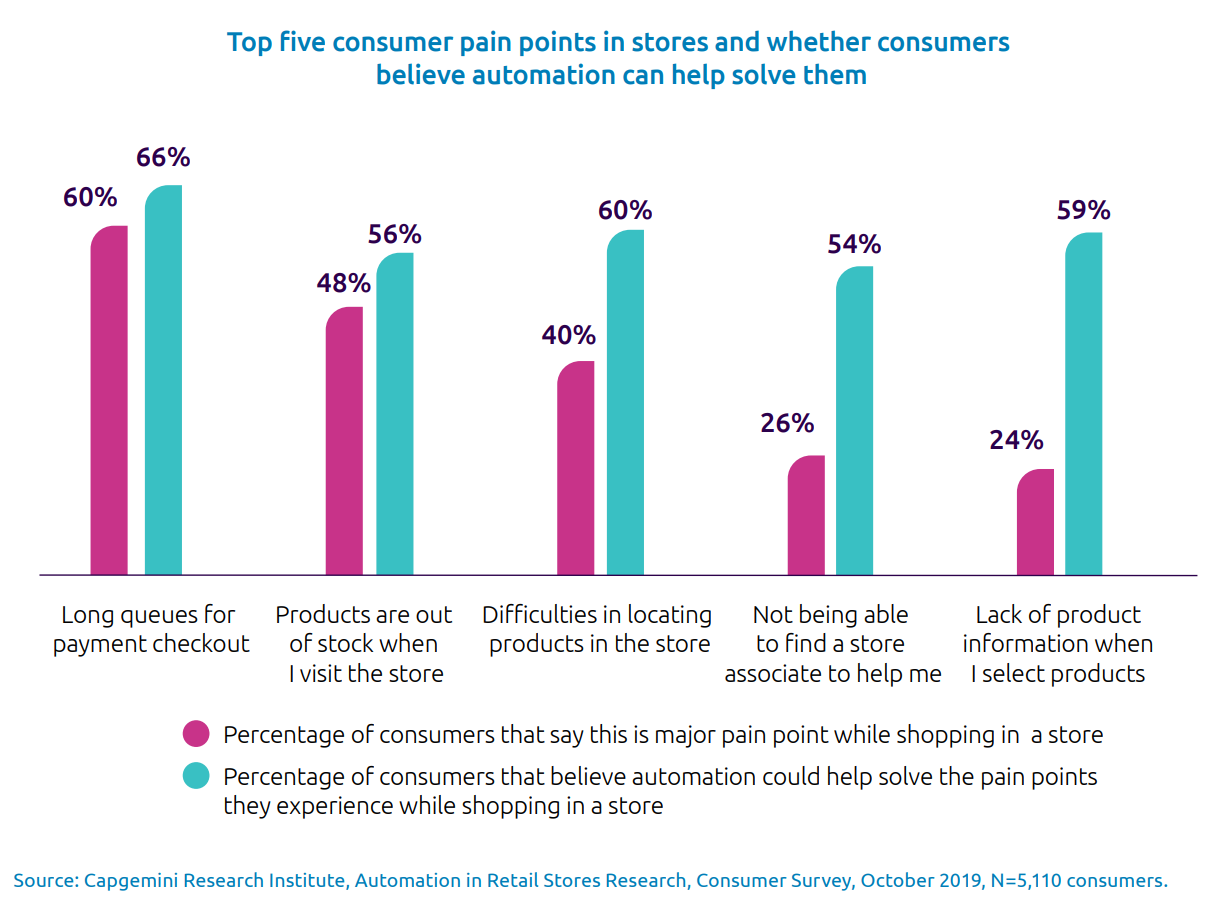
\includegraphics[width=0.8\textwidth]{./images/painpoints.png}
    \fonte{\cite{Capgemini2020}}
    \label{fig:capgemini}
\end{figure}

More interestingly, the survey points out that at least half of the survey
respondents believe that all of the five pain points can be solved through
\textbf{automation}. Even in light of the recent pandemic scenario, innovations
that increase automation such as e-commerce platforms had their adoption
increased in 2020 but 2021 showed a trend of consumers shifting
back to their pre-pandemic behavior, favoring physical retail stores
\cite{Kantar2022}.

It is in this scenario of customer pain and enormous market potential that this
thesis will explore a technological solution to improve customer experience and increase sales,
namely the \textbf{smart shopping cart}.

\section{Current scenario}

In this next section, we'll explore some of the existing solutions and the user experience
provided by them.

\subsection{Caper Cart}

Developed by the Caper\footnote{https://caper.ai} company, the Caper Cart was the worlds's first AI-powered smart cart \cite{Caper2020}

The first version was launched in 2017 and offered grocer's the
great advantage of not requiring any infrastructure overhaul for deployment.
In Figure \ref{fig:caperatretail}, we can see the cart deployed at American
retail store.

\begin{figure}[H]
	\centering
	\caption[Caper Cart at a retail store]{Caper Cart at a retail store}
	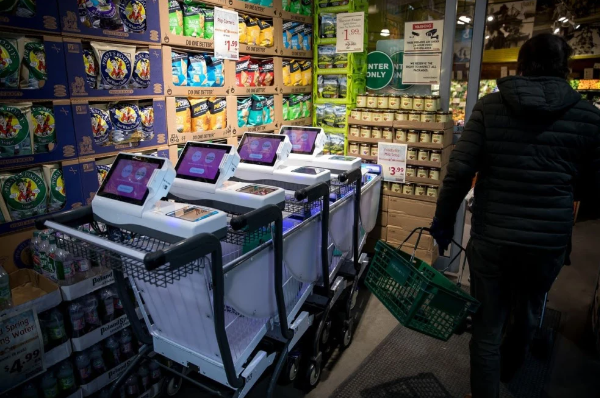
\includegraphics[width=0.7\textwidth]{./images/caper.png}
    \fonte{Caper (2020)}
	\label{fig:caperatretail}
\end{figure}

For end users, it offered visual product recognition and a payment terminal,
allowing them to avoid the dreaded queues by the end of their shopping session.
Additionally, customers were able to search products, get discounts and locate
items more easily with the help of the interactive user interface provided by the cart that 
can be seen on Figure \ref{fig:caperui}.

\begin{figure}[H]
	\centering
	\caption[Caper Cart user interface]{Caper Cart user interface}
	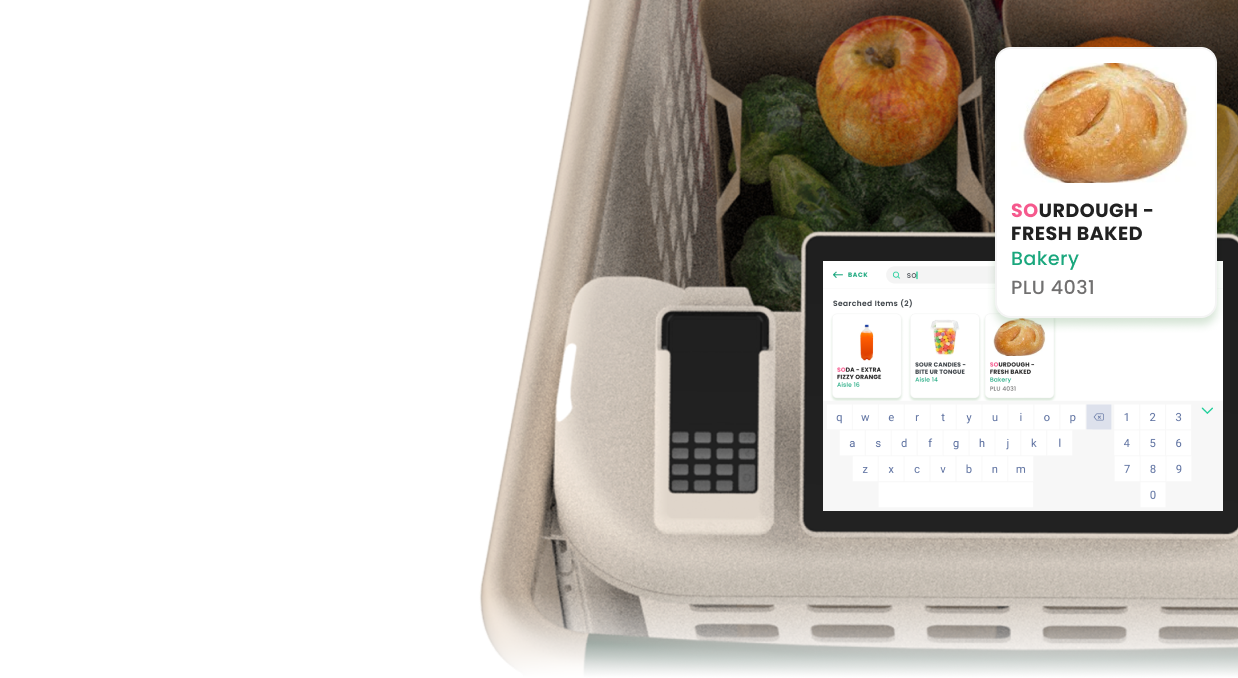
\includegraphics[width=0.7\textwidth]{./images/capercartui.png}
    \fonte{Caper (2020)}
	\label{fig:caperui}
\end{figure}

Although Caper does not publicize the cost of each cart, it is estimated that each unit costs between
\textbf{US\$ 5,000 and 10,000} \cite{TWP2021}.

Acquired by Instacart\footnote{https://instacart.com} in 2021 for US\$ 350
million, Caper is developing in 2022 the third version of its Smart Shopping
Cart, advertising an increase of \textbf{65\% in the basket volume} and a
\textbf{10 month} break even period, as shown on Figure \ref{fig:caperad}.

\begin{figure}[H]
	\centering
	\caption[Caper Cart 3 promotional material]{Caper Cart 3 promotional material}
	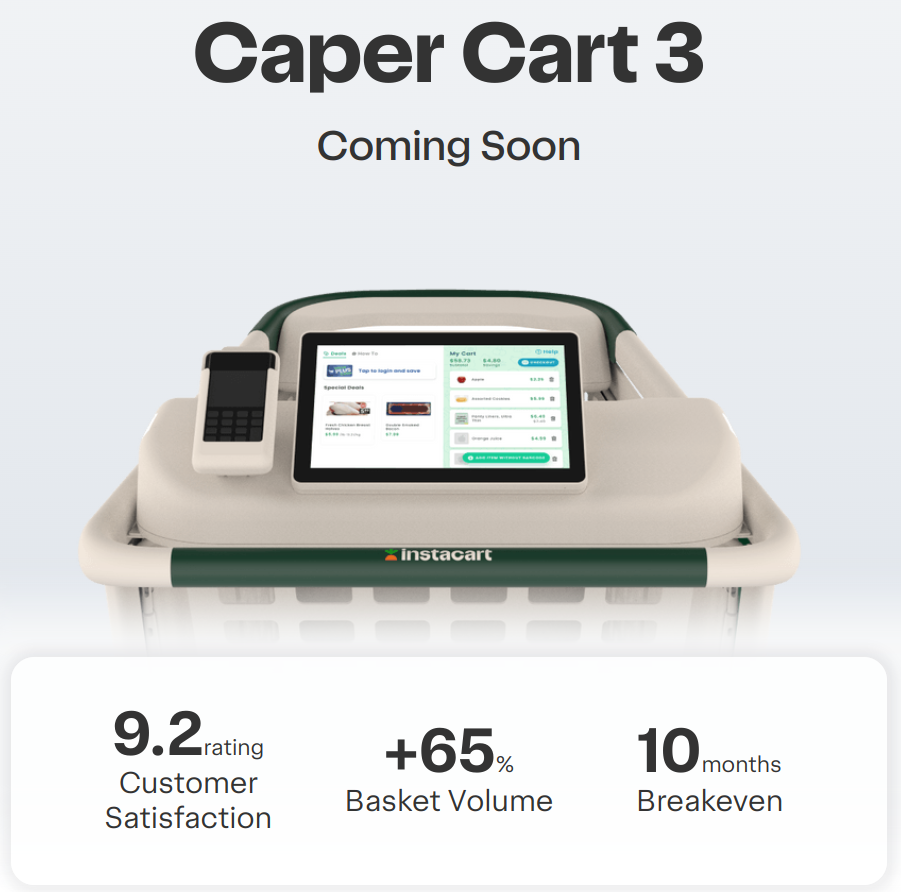
\includegraphics[width=0.7\textwidth]{./images/capercart3.png}
    \fonte{Caper (2022)}
	\label{fig:caperad}
\end{figure}


\subsection{Amazon Dash Cart}

Available at the Amazon Fresh\footnote{https://www.amazon.com/fmc/m/30003175?almBrandId=QW1hem9uIEZyZXNo} retail chain, the
Amazon Dash Cart is the company's first smart cart available to end users and is shown in
Figure \ref{fig:dashcart}.

According to Amazon, it uses computer vision and sensors to allow customers to
simply add items to their cart like they usually would. The cart accounts all
the items present in the cart, displaying a list which includes their prices
and subtotal. By the end of their item selection, customers can check-out
automatically without having to go through queues, solving the biggest customer
pain point pointed out by \cite{Capgemini2020}.

\begin{quote}
\textit{Looking to make grocery trips quicker? With the Amazon Dash Cart you can skip the checkout line and roll out to your car when you are done.}

\textit{The Dash cart uses a combination of computer vision algorithms and sensor fusion to help identify items placed in the cart - simply grab an item, scan it on one of the Dash Cart cameras, and place it in the cart like you normally would.}
\\
Amazon (2022)
\end{quote}

\begin{figure}[H]
	\centering
    \caption[Amazon Dash Cart]{Amazon Dash Cart}
	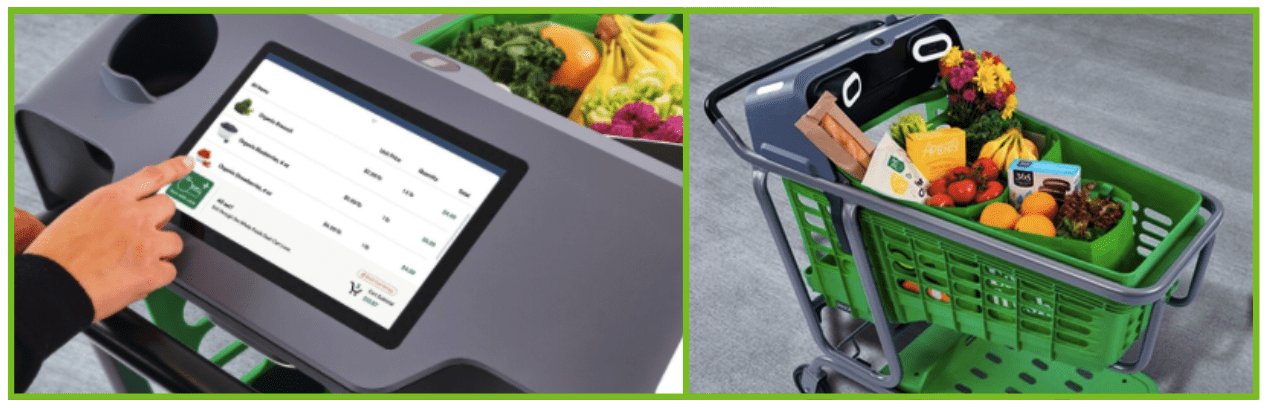
\includegraphics[width=0.8\textwidth]{./images/dashcart.png}
    \fonte{Amazon (2022)}
    \label{fig:dashcart}
\end{figure}

In addition to the item accounting capabilities, the user interface provided by
the Cart also allows customers to search for the location of items  in the
store and see more information about them, improving the customer experience.

One of its particularities is that it requires the download and usage of an mobile phone
app for using the cart, something not required by Caper's Cart.

As of October 2022, the Amazon Dash Cart is exclusively available at the Amazon
Fresh chain and therefore no commercial information regarding cost per unit is
available.

\subsection{Nextop}

Founded in 1997, Nextop\footnote{https://nextop.com.br} is a Brazilian company
that develops products with a focus on the grocery stores market, with an emphasis on
loss prevention.

Their smart cart offering, shown in Figure \ref{fig:nextop}, is the first
deployed in Brazil and Latin America according to the company and was
initially rolled out to the Enxuto supermarket chain in 2022
\cite{Paraiba2022}.

\begin{figure}[H]
	\centering
	\caption[Smart Cart Nextop® deployed to a Brazilian supermarket]{Smart Cart Nextop® deployed to a Brazilian supermarket}
	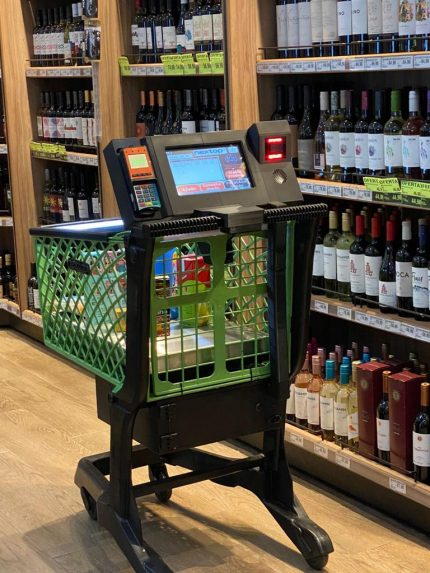
\includegraphics[width=0.4\textwidth]{./images/nextop.jpeg}
    \fonte{Nextop (2022)}
	\label{fig:nextop}
\end{figure}

In contrast to the carts developed by Amazon and Caper, Nextop's cart requires
an additional step of scanning the product using the integrated barcode reader,
shown in Figure \ref{fig:nextopui}, before adding it to the cart. With that, the
Nextop advertises for a \textit{triple validation} system, using the cameras,
sensors and the barcode scanner to prevent losses \cite{Nextop2022}.

\begin{figure}[H]
	\centering
    \caption[Smart Cart Nextop® user interface with a payment terminal]{Smart Cart Nextop® user interface with a payment terminal}
	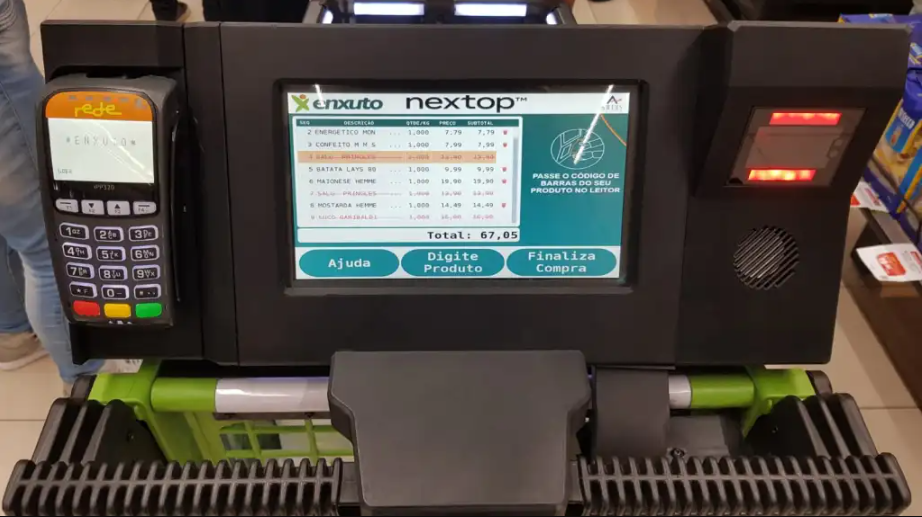
\includegraphics[width=0.9\textwidth]{./images/nextop2.png}
    \fonte{\cite{Paraiba2022}}
	\label{fig:nextopui}
\end{figure}

Although loss prevention is an important selling point for the Brazilian market,
the usage of the barcode scanner creates, in our opinion, a worse customer
experience, becoming a \textit{mobile checkout station}. Also, the product does not
include additional features such as product location search and item details. 

Figure \ref{fig:nextopad} shows an advertisement, in Portuguese, that lists the following
benefits:

\begin{itemize}
    \item Innovative supermarkets sell 20\% more
    \item Loss prevention
    \item Triple validation
    \item Freedom and agility
    \item New self checkout using artificial intelligence
    \item No queues
\end{itemize}

\begin{figure}[H]
	\centering
    \caption[Smart Cart Nextop® promotional material targetting supermarket owners]{Smart Cart Nextop® promotional material targeting supermarket owners. It advertises for improved sales, loss prevention and reduced queues.}
	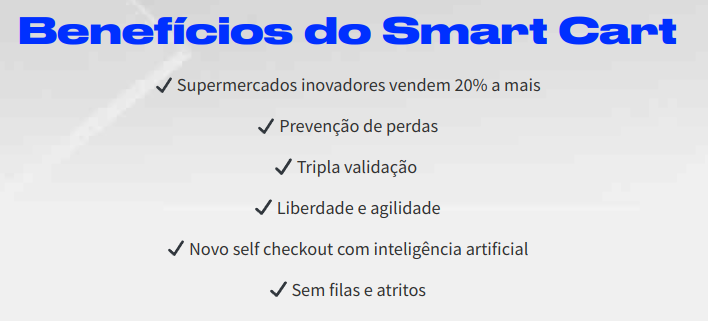
\includegraphics[width=0.9\textwidth]{./images/nextoppromo.png}
    \fonte{\cite{Nextop2022}}
	\label{fig:nextopad}
\end{figure}

Offering a solution to the main end user pain point of having to go through
long queues, the product also advertises increased sales as a result of the
innovative approach and also allows a deeper understanding of the customer
journey by collecting analytical data \cite{Paraiba2022}.

\begin{quote}
\textit{We are offering our customers an innovative and unique shopping experience within Enxuto}

\textit{With the smart cart, we broke through this barrier and managed to monitor the
entire customer's purchase circuit in the physical store. We have moved
from the identified ticket era to the end-to-end identified journey}

    Bruno Bragancini Junior, \sigla{CEO}{Chief Executive Officer} of the Enxuto Group \cite{Paraiba2022}
\end{quote}

According to Nextop's CEO, Juliano Camargo, the company has already invested \textbf{R\$ 8,5 millions} - about US\$ 1,63 million on October 2022 - and \textbf{4 and half years}
of research and development.

Each Smart Cart is estimated to cost around \textbf{R\$ 120,000} or around US\$ 23,020 on October 2022 \cite{Paraiba2022}.

\section{Objectives}

After presenting the problem domain and the current market scenario, in this section we discuss the 
objectives of this work.

\subsection{Main objective}
Develop a prototype of a smart shopping cart that utilizes computer
vision and sensor data for product recognition.

\subsection{Specific objectives}
\begin{itemize}
    \item Build a mechanical assembly for the prototype
    \item Develop an interactive user interface for the prototype
    \item Collect a product dataset for training a deep learning model
    \item Train a Deep Learning model capable of detecting target products
	\item Learn the practical challenges of developing a Deep Learning based product
    \item Understand the economic viability of such a project in the Brazilian context
\end{itemize}
